\subsection{Khảo sát thị trường}
\subsubsection{CellphoneS}
\begin{figure}[H]
    \centering
    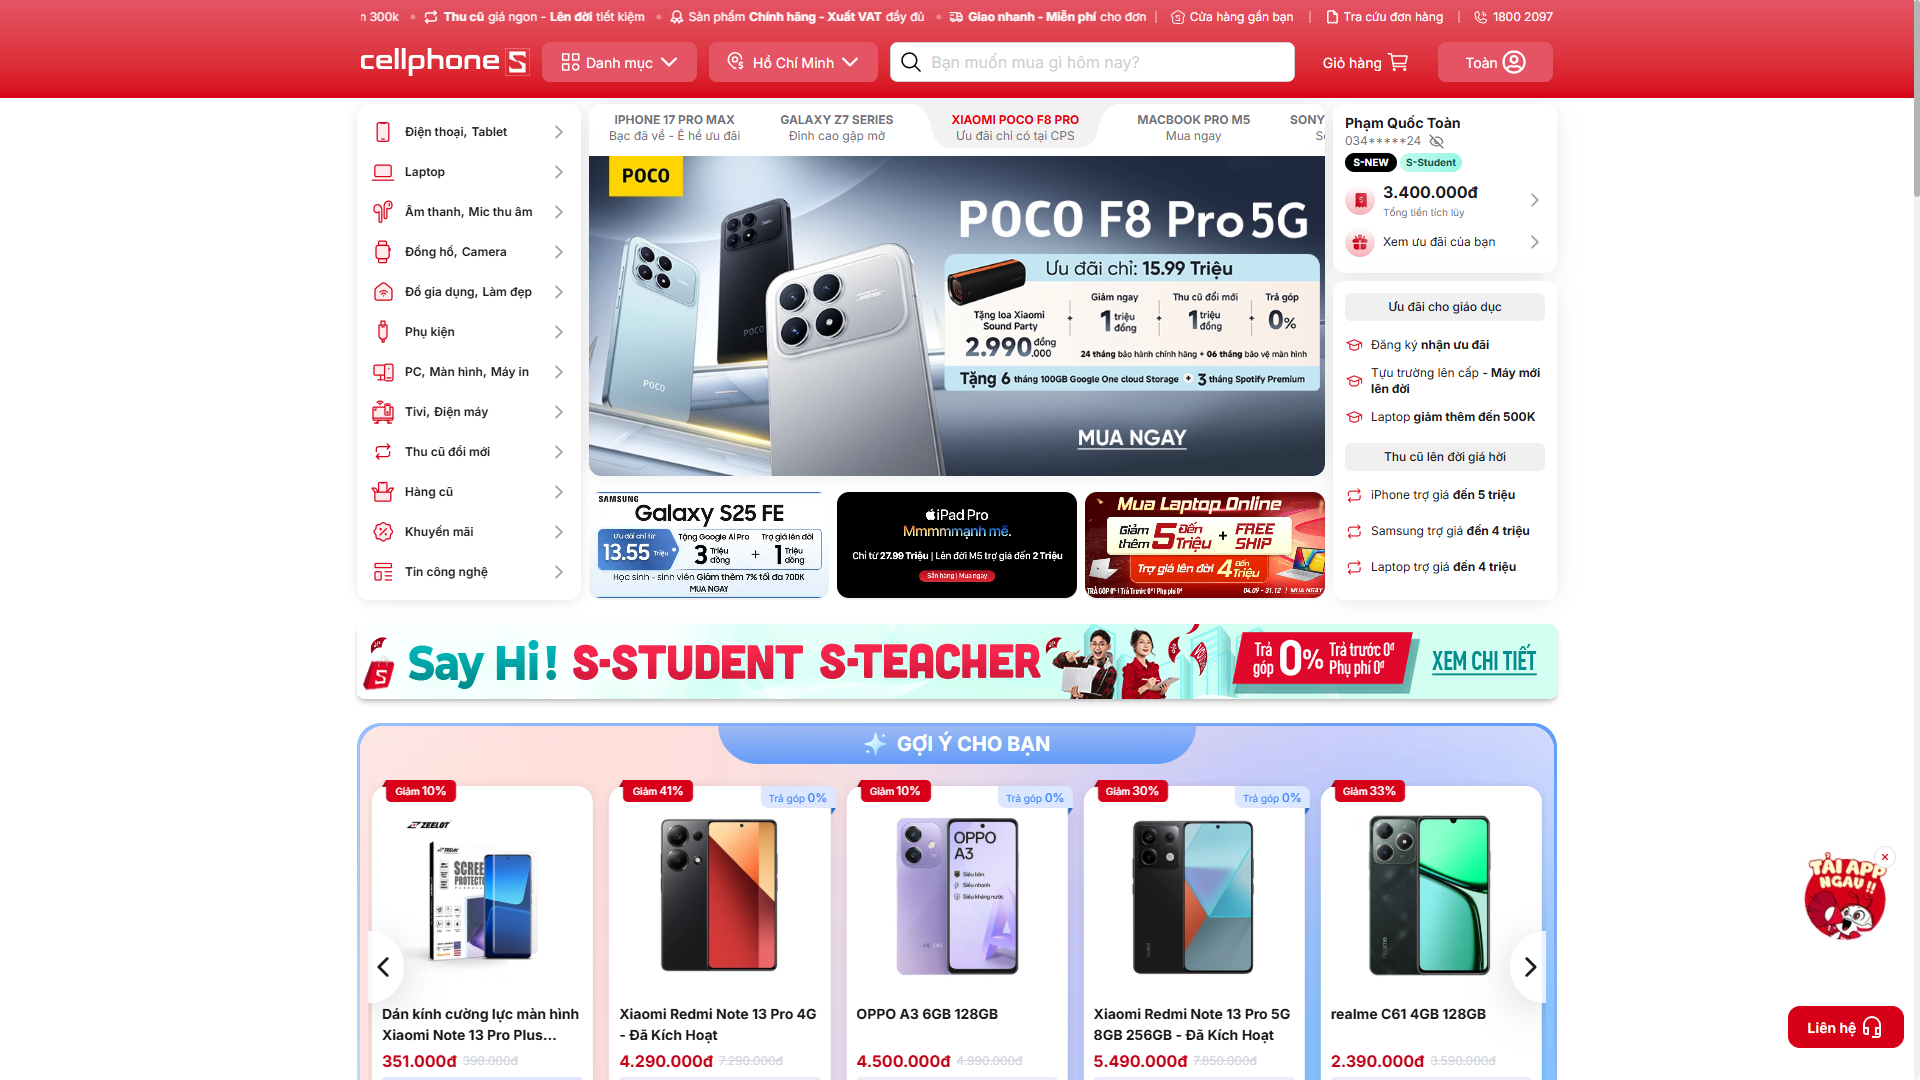
\includegraphics[width=\textwidth]{images/chap2/cellphones.png}
    \vspace{0.5cm}
    \caption{Trang chủ của CellphoneS}
\end{figure}

CellphoneS là hệ thống bán lẻ điện thoại, laptop, máy tính bảng và nhiều phụ kiện công nghệ phổ biến tại Việt Nam, hoạt động song song giữa chuỗi cửa hàng và nền tảng thương mại điện tử. Website của CellphoneS hướng tới trải nghiệm mua sắm nhanh, tiện lợi, hỗ trợ trả góp, chương trình thu cũ đổi mới (trade-in) và hệ thống tích điểm khách hàng thân thiết Smember.

\textbf{Tính năng nổi bật:}
\begin{itemize}
    \item Bộ lọc và tìm kiếm sản phẩm theo giá, thương hiệu, thông số kỹ thuật và chương trình khuyến mãi.
    \item Hỗ trợ trade-in với quy trình định giá trực tuyến và phản hồi nhanh.
    \item Trả góp linh hoạt qua nhiều hình thức như thẻ tín dụng, công ty tài chính hoặc ví điện tử.
    \item Ứng dụng Smember giúp người dùng quản lý điểm thưởng, theo dõi ưu đãi và thông báo khuyến mãi.
\end{itemize}

Website của CellphoneS thể hiện thế mạnh rõ rệt ở việc xây dựng quy trình trade-in minh bạch và dễ sử dụng, cùng với hệ thống trả góp linh hoạt, giúp người dùng có nhiều lựa chọn tài chính phù hợp. Nền tảng Smember tạo ra hệ sinh thái khách hàng thân thiết, góp phần giữ chân người dùng lâu dài. Tuy nhiên, website vẫn còn hạn chế ở khả năng cá nhân hóa trải nghiệm mua sắm. Các tính năng như đề xuất sản phẩm thông minh hay chatbot hỗ trợ tương tác tự nhiên chưa được đầu tư sâu, khiến hệ thống vẫn chủ yếu hoạt động theo cơ chế tìm kiếm và thao tác thủ công.



\subsubsection{FPT Shop}
\begin{figure}[H]
    \centering
    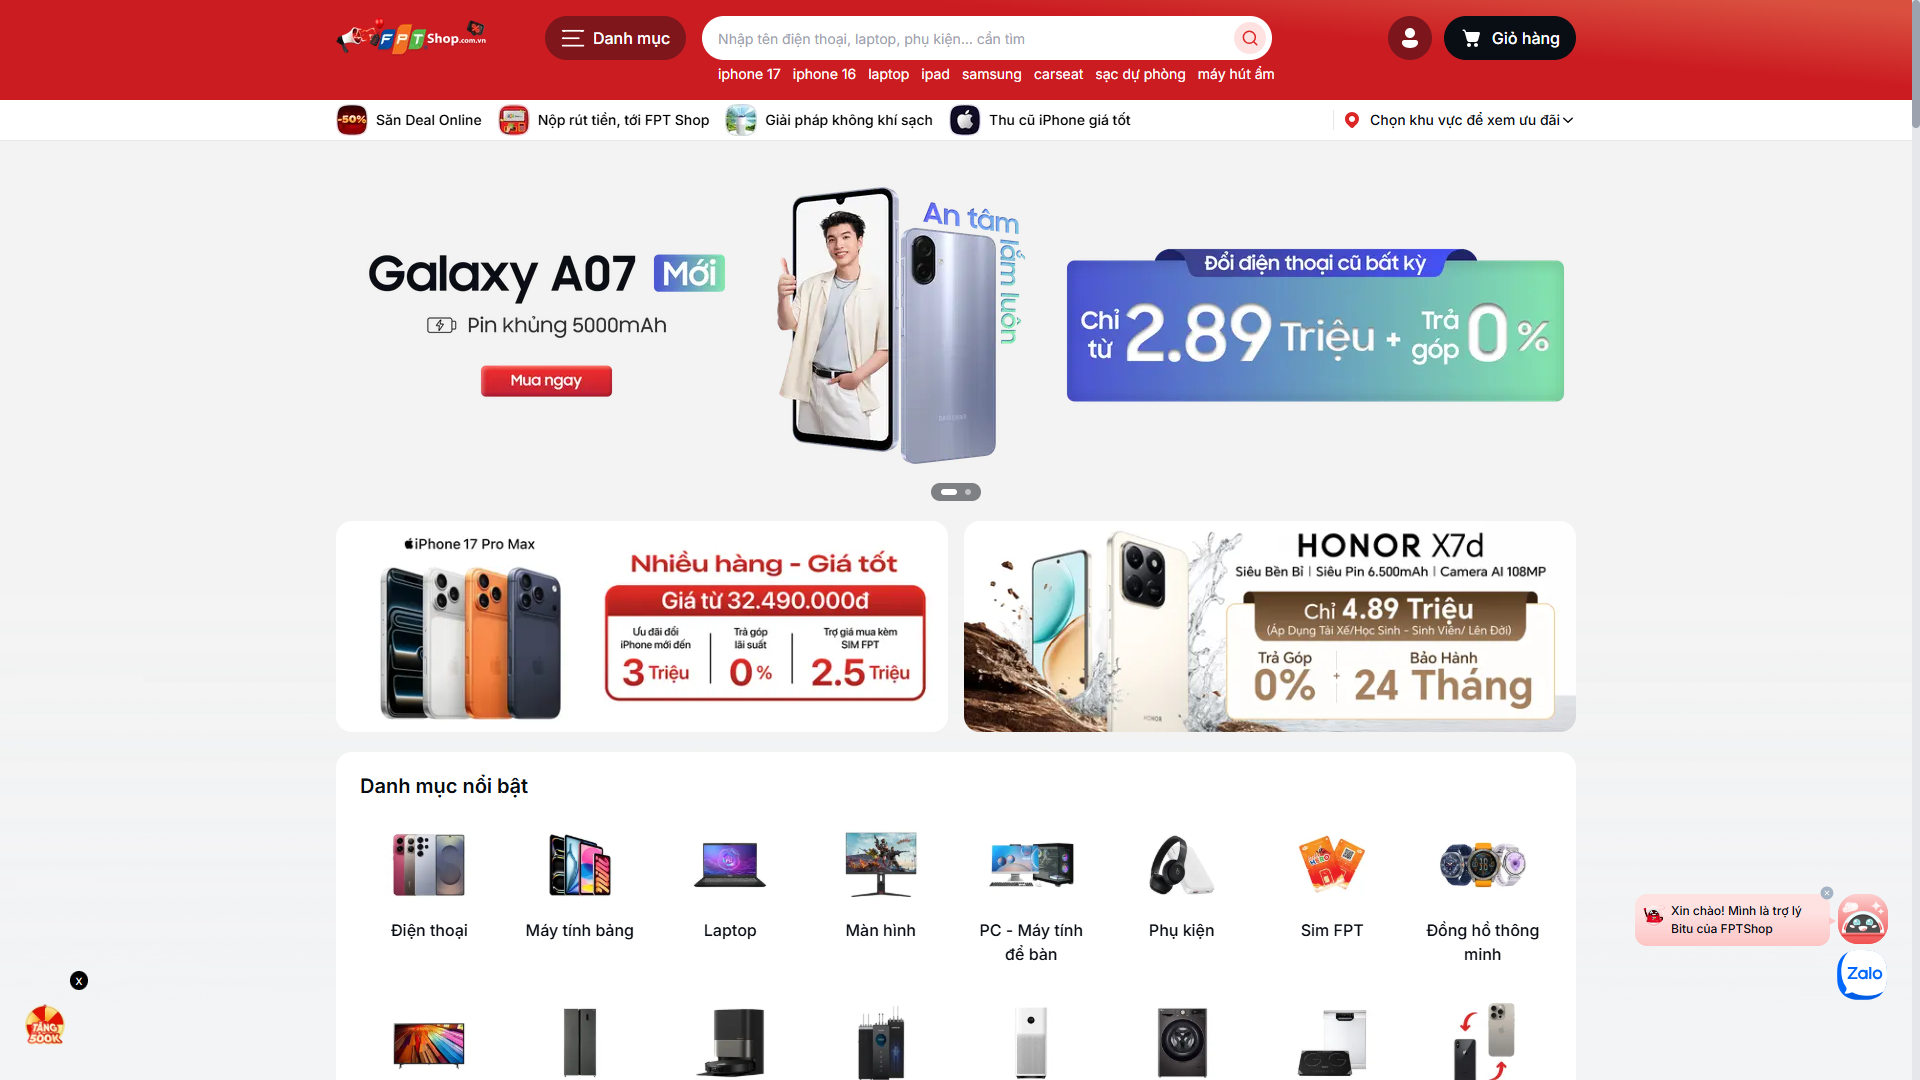
\includegraphics[width=\textwidth]{images/chap2/fpt.png}
    \vspace{0.5cm}
    \caption{Trang chủ của FPT Shop}
\end{figure}

FPT Shop là thương hiệu bán lẻ thiết bị công nghệ thuộc Tập đoàn FPT, với mạng lưới cửa hàng rộng khắp và nền tảng thương mại điện tử tích hợp mạnh mẽ. Website của FPT Shop chú trọng trải nghiệm người dùng, hỗ trợ trả góp, khuyến mãi và dịch vụ hậu mãi, đồng thời ứng dụng công nghệ AI trong tư vấn, hỗ trợ khách hàng.

\textbf{Tính năng nổi bật:}
\begin{itemize}
    \item Hệ thống tìm kiếm và lọc sản phẩm mạnh, hiển thị nhiều biến thể sản phẩm và cho phép so sánh cơ bản.
    \item Hỗ trợ trả góp đa dạng với thông tin minh bạch về lãi suất và các tùy chọn thanh toán.
    \item Ứng dụng di động cung cấp thông tin khuyến mãi, voucher và tích điểm khách hàng thân thiết.
\end{itemize}

FPT Shop sở hữu nền tảng công nghệ hiện đại với khả năng đồng bộ tốt giữa kênh bán hàng trực tuyến và hệ thống cửa hàng vật lý, mang lại trải nghiệm mua sắm liền mạch cho người dùng. Website cung cấp đầy đủ các chức năng như tra cứu sản phẩm, xem thông tin chi tiết, so sánh và đặt hàng trực tuyến, đáp ứng hiệu quả nhu cầu mua sắm của khách hàng.

Tuy nhiên, hệ thống hiện chưa tích hợp trợ lý ảo hoặc chatbot thông minh trên nền tảng web để hỗ trợ người dùng trong quá trình tương tác. Việc hỗ trợ khách hàng chủ yếu vẫn dựa vào các kênh truyền thống như tổng đài hoặc tư vấn viên trực tuyến. Cách tiếp cận này giúp đảm bảo độ chính xác trong phản hồi, nhưng đồng thời làm hạn chế khả năng tự động hóa và phản hồi nhanh, đặc biệt khi số lượng người dùng tăng cao.

Bên cạnh đó, việc thiếu một hệ thống trợ lý ảo cũng khiến trải nghiệm người dùng vẫn mang tính thụ động, phụ thuộc vào thao tác tìm kiếm và điều hướng thủ công. Điều này cho thấy tiềm năng ứng dụng trí tuệ nhân tạo trong việc hỗ trợ tư vấn, so sánh sản phẩm và giải đáp thắc mắc vẫn chưa được khai thác hiệu quả trong hệ thống.



\subsubsection{Thế Giới Di Động}
\begin{figure}[H]
    \centering
    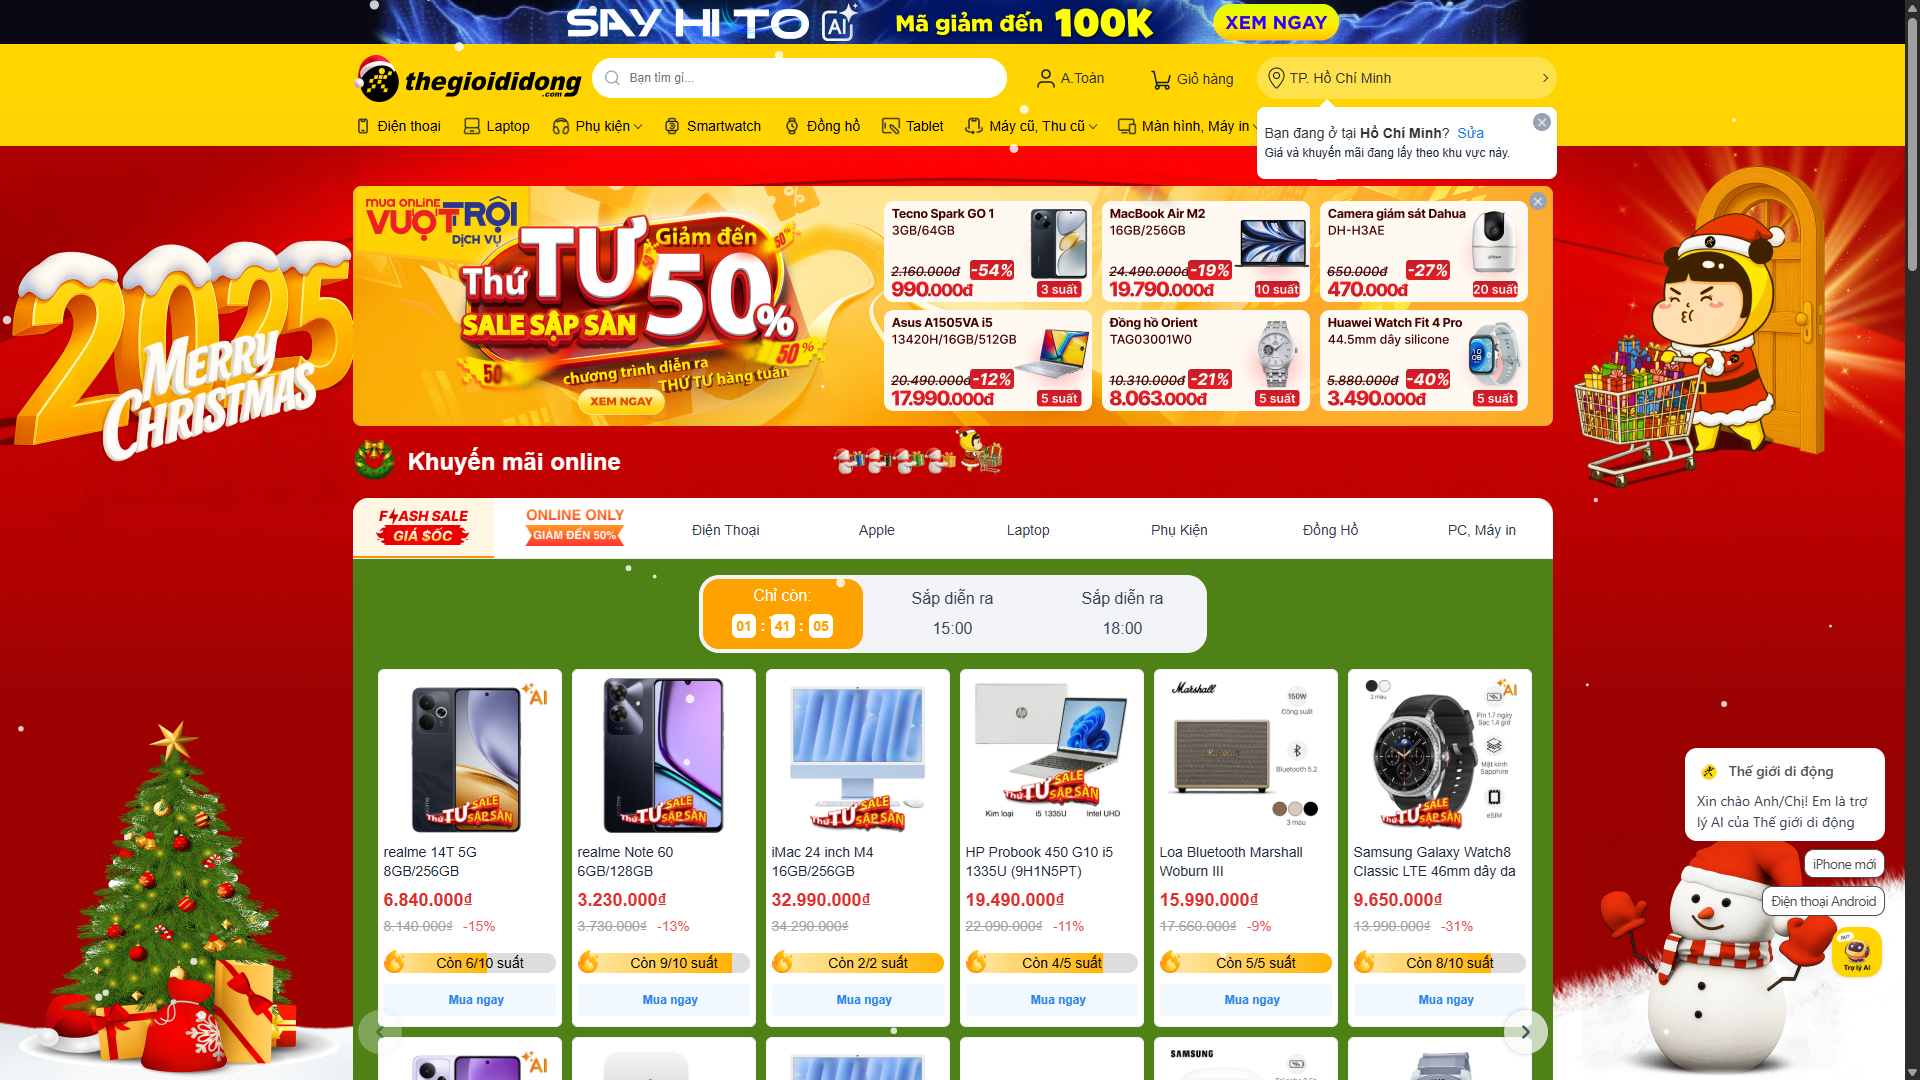
\includegraphics[width=\textwidth]{images/chap2/tgdd.png}
    \vspace{0.5cm}
    \caption{Trang chủ của Thế Giới Di Động}
\end{figure}

Thế Giới Di Động là hệ thống bán lẻ điện thoại và thiết bị điện tử tiêu dùng lớn nhất Việt Nam, với hàng nghìn cửa hàng trên toàn quốc. Website được tối ưu cho người dùng phổ thông, tập trung vào quy trình mua nhanh, khuyến mãi hấp dẫn và chính sách hậu mãi rõ ràng.

\textbf{Tính năng nổi bật:}
\begin{itemize}
    \item Bộ lọc sản phẩm đa tiêu chí, gợi ý kết quả tức thì và hiển thị sản phẩm nổi bật.
    \item Chính sách giao hàng, đổi trả, bảo hành minh bạch.
    \item Hệ thống khuyến mãi, flash sale và combo sản phẩm trình bày nổi bật.
    \item Hỗ trợ khách hàng đa kênh: hotline, chat trực tuyến, mạng xã hội và cửa hàng.
\end{itemize}

Website của Thế Giới Di Động có thiết kế thân thiện, tốc độ truy cập cao và khuyến mãi cập nhật liên tục. Bên cạnh đó, Thế Giới Di Động đã tích hợp trợ lý ảo hỗ trợ khách hàng. Tuy nhiên, các trợ lý ảo này chỉ dừng lại ở mức trả lời câu hỏi hoặc hướng dẫn cơ bản. Các trợ lý ảo này chưa làm tốt trong việc duy trì một luồng hỗ trợ khách hàng nhiều lượt và phi tuyến tính.

\begin{figure}[H]
\centering
\begin{minipage}{0.30\textwidth}
    \centering
    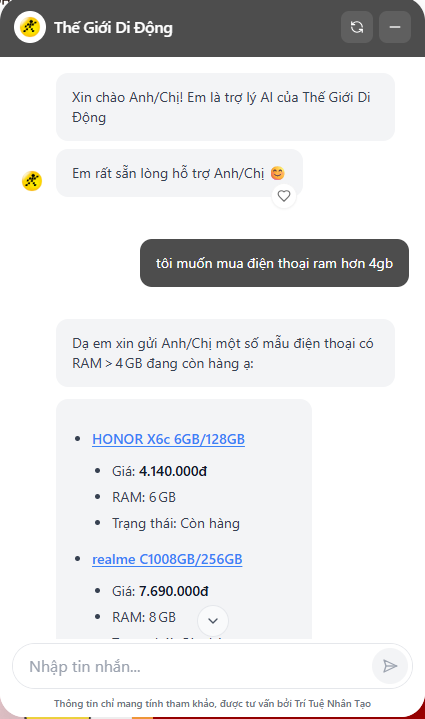
\includegraphics[width=0.8\textwidth]{images/chap2/tgdd_good.png}
\end{minipage}
\hfill
\begin{minipage}{0.30\textwidth}
    \centering
    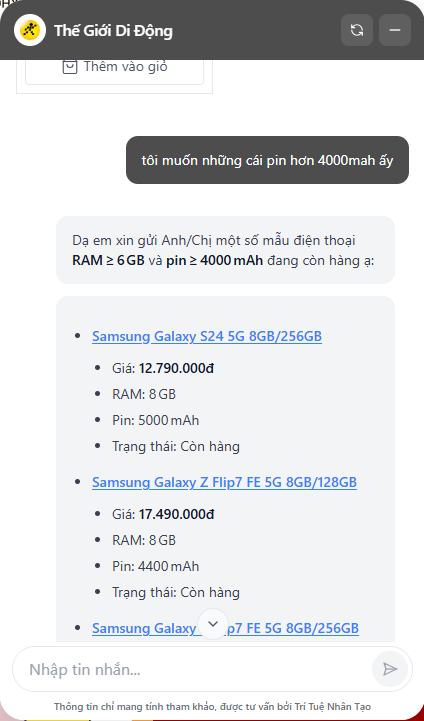
\includegraphics[width=0.8\textwidth]{images/chap2/tgdd_bad1.png}
\end{minipage}
\hfill
\begin{minipage}{0.30\textwidth}
    \centering
    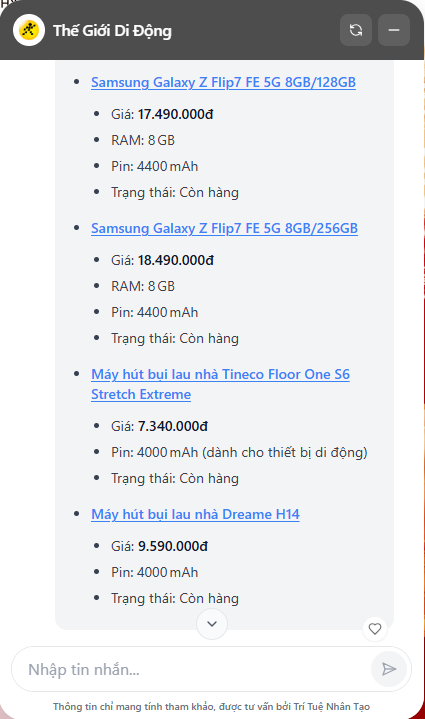
\includegraphics[width=0.8\textwidth]{images/chap2/tgdd_bad2.png}
\end{minipage}
\vspace{0.5cm}
\caption{Trợ lý ảo của Thế Giới Di Động}
\end{figure}



\subsubsection{So sánh tính năng giữa các nền tảng hiện có và hệ thống đề xuất}

\begin{table}[H]
\centering
\caption{So sánh tính năng giữa các nền tảng hiện có và hệ thống đề xuất}
\renewcommand{\arraystretch}{1.5}
\begin{tabular}{|p{5.5cm}|c|c|c|c|}
\hline
\textbf{Nhóm tính năng} & \textbf{CellphoneS} & \textbf{FPT Shop} & \textbf{Thế Giới Di Động} & \textbf{Hệ thống đề xuất} \\
\hline
Tìm kiếm và lọc sản phẩm & Có & Có & Có & Có \\
\hline
Phân loại và hiển thị sản phẩm & Có & Có & Có & Có \\
\hline
Đánh giá và phản hồi sản phẩm & Có & Có & Có & Có \\
\hline
Quản lý giỏ hàng và đơn hàng & Có & Có & Có & Có \\
\hline
Hệ thống khuyến mãi và ưu đãi & Có & Có & Có & Có \\
\hline
Giao diện thân thiện, tối ưu UX/UI & Có & Có & Có & Có \\
\hline
Tư vấn sản phẩm & Không & Không & Hạn chế & Thông minh \\
\hline
\end{tabular}
\renewcommand{\arraystretch}{1.0}
\end{table}

Từ kết quả khảo sát ba nền tảng thương mại điện tử lớn tại Việt Nam, có thể nhận thấy rằng mỗi hệ thống đều có định hướng riêng trong việc phát triển và phục vụ người dùng.

Tuy nhiên, nhóm nhận thấy rằng mặc dù các doanh nghiệp trong ngành đã có bước tiến lớn trong việc số hóa hoạt động bán lẻ, các nền tảng thương mại điện tử trong mảng bán lẻ điện thoại di động và các đồ dùng công nghệ tại Việt Nam chưa thật sự tích hợp Trợ lý Ảo thông minh có khả năng giao tiếp tự nhiên và duy trì luồng hỗ trợ nhiều lượt và phi tuyến tính.

Khoảng trống này mở ra cơ hội để nhóm nghiên cứu và phát triển một mô hình thương mại điện tử tích hợp Trợ lý Ảo AI Agent, hướng đến việc nâng cao trải nghiệm người dùng, tự động hóa quy trình giao dịch, và tăng tính cá nhân hóa trong tương tác mua sắm.
